\documentclass{article}

\usepackage{a4}
\usepackage{amsmath}
\usepackage{amssymb}
\usepackage{ctex}
\usepackage{booktabs}
\usepackage{graphicx}
\usepackage{subfigure}
\usepackage{subcaption}
\usepackage{float}
\usepackage{hyperref}
\usepackage{xurl}
\usepackage{enumitem}
\usepackage{array}
\usepackage{longtable}
\usepackage{multirow}
\usepackage{fvextra}

\hypersetup{colorlinks=true,linkcolor=black,urlcolor=blue,citecolor=black}
\setlist[itemize]{nosep,leftmargin=1.8em}
\setlist[enumerate]{nosep,leftmargin=1.8em}
\captionsetup{font=small}
\RecustomVerbatimEnvironment{verbatim}{Verbatim}{
  breaklines=true,
  breakanywhere=true,
  fontsize=\small
}

\title{计算机组成原理\\大作业\\多周期与五级流水线CPU的复现与改进}
\author{鲁昕宁 2414015}
\date{\today}

\begin{document}

\maketitle
\begin{center}
    \url{https://github.com/SidneyLu/Computer-Organization-and-Design-NKU-CS/tree/master/final_project}
\end{center}

\newpage

\section{实验目标}
1.找到多周期和五级流水线CPU原始代码和方案中存在的bug并修复，
详细说明bug发现过程和修复过程及效果，保证现有的coe中汇编程序执行正确。

2.仿照单周期CPU实验，自行用MIPS汇编写一个完整具体的计算任务，
把这个计算任务放到coe中交给流水线CPU执行。注意，在流水线执行过程中会出现
数据相关等情况，自行选择方案解决数据冲突（三个方案，分别是填充空指令、流水线阻塞、前递与旁路）。

\section{实验原理}
\begin{figure}[h!]
  \centering
  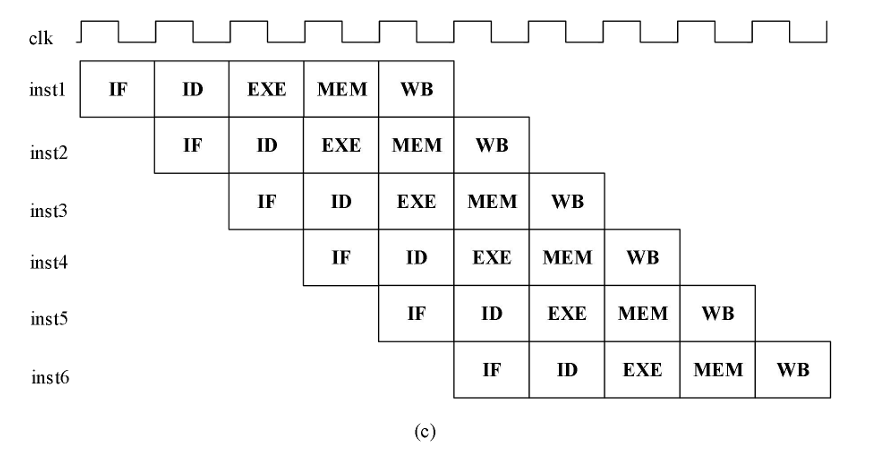
\includegraphics[width=\textwidth]{pipeline.png}
  \caption{5级流水线CPU时空图}
\end{figure}

流水线（Pipeline）的引入是计算机体系结构发展史上的一次跃进。
它的核心意义可以从以下几个维度来理解：
1. 核心意义：极大提升 CPU 的吞吐量（Throughput）

在没有流水线的设计中（如单周期或多周期 CPU），
一条指令必须完整地经历“取指（IF） $\rightarrow$ 译码（ID） $\rightarrow$ 执行（EX） $\rightarrow$ 访存（MEM） $\rightarrow$ 写回（WB）”
这五个阶段，下一条指令才能开始。
这意味着在某一时刻，CPU 只有一小部分电路在工作，其余大部分硬件都在“闲置”。
而引入流水线后，指令级并行程度得到提升：
当第一条指令在执行（EX）时；第二条指令正在译码（ID）；
第三条指令已经开始取指（IF）。
当然流水线并没有缩短单条指令的执行时间（延迟 Latency），
甚至由于增加了流水线寄存器，单条指令的延迟还会略微增加。
但它让 CPU 在单位时间内能够完成的指令总数（吞吐量）呈倍数级增长。
在理想状态下，每个时钟周期都能“吐出”一条执行完的指令。

2. 性能质变：拉高主频（Clock Frequency）

评估 CPU 性能有一个公式：
$$\text{CPU Time} = \text{Instruction Count} \times \text{CPI} \times \text{Clock Cycle Time}$$$\text{CPI}$：每条指令所需的平均时钟周期数。$\text{Clock Cycle Time}$：时钟周期（主频的倒数），由电路中最长的那条路径（关键路径）的延时决定。
在多周期 CPU 中，为了让复杂的指令在单个时钟周期内不至于拖慢整体速度，状态机和控制逻辑会变得极其繁琐；
而在单周期 CPU 中，时钟周期必须满足最慢的那条指令（通常是 lw），导致主频根本无法提升。
流水线把一条复杂的指令切分成 5 个（或更多）近似均等的微小阶段。
时钟周期不再取决于整条指令的长度，而仅仅取决于这 5 个阶段中最慢的那一个阶段的延时。
这种“化整为零”的切分，让关键路径大大缩短，
使得 CPU 的时钟频率（主频）可以轻松提升。

3. 硬件资源利用率（Hardware Utilization）最大化

执行 addiu 的 ALU 运算时，内存控制部件（Memory）完全在闲置。  
执行 lw 访存时，ALU 运算部件又在闲置。  
流水线设计让算术逻辑单元（ALU）、指令寄存器（IR）、
数据存储器（Data Memory）和寄存器堆（Register File）
在每一个时钟周期都处于全负荷运转状态。
这种高强度的硬件复用，用最经济的芯片面积换取了最大的算力输出。

4. 催生了现代高端 CPU 技术

流水线是所有现代高性能高级处理器技术的“入场券”。没有流水线，以下技术都无从谈起：超流水线（Super-pipelining）： 将 5 级流水线继续细拆成 14 级甚至 31 级（如 Intel Pentium 4），把主频榨干到极致。超标量（Superscalar）： 
既然一条流水线不够用，那就并行摆放多条流水线，实现每个周期同时发射、同时执行多条指令（现代 PC 处理器多为 4-6 发射）。
乱序执行（Out-of-Order Execution）与分支预测（Branch Prediction）： 专门为了解决流水线“卡顿”（冒险/冲突）而衍生出的顶级硬件优化技术。


当然，世界上没有免费的午餐。流水线伴随着“冒险（Hazards）”：
\begin{itemize}
  \item 结构冒险：多个阶段同时争抢同一个硬件（如同时读写内存）。
  \item 数据冒险：后一条指令要用到前一条指令还没写回的脏数据（数据冲突）  
  \item 控制冒险：遇到 beq、bgez 等跳转指令时，CPU 不知道该继续取哪里的指令
\end{itemize}
以上冒险导致流水线不得不面临“刷洗（Flush）”或“阻塞（Stall）”的惩罚  
现代CPU很大一部分设计精力，其实都倾注在享受流水线高吞吐量的同时，
弥补这些由流水线带来的副作用，如多发射、乱序执行、分支预测等。

\newpage
\section{实验过程}
\subsection{IP核创建}
按照实验指导手册说明创建指令ROM和数据RAM的IP核。
\begin{figure}[h!]
  \centering
  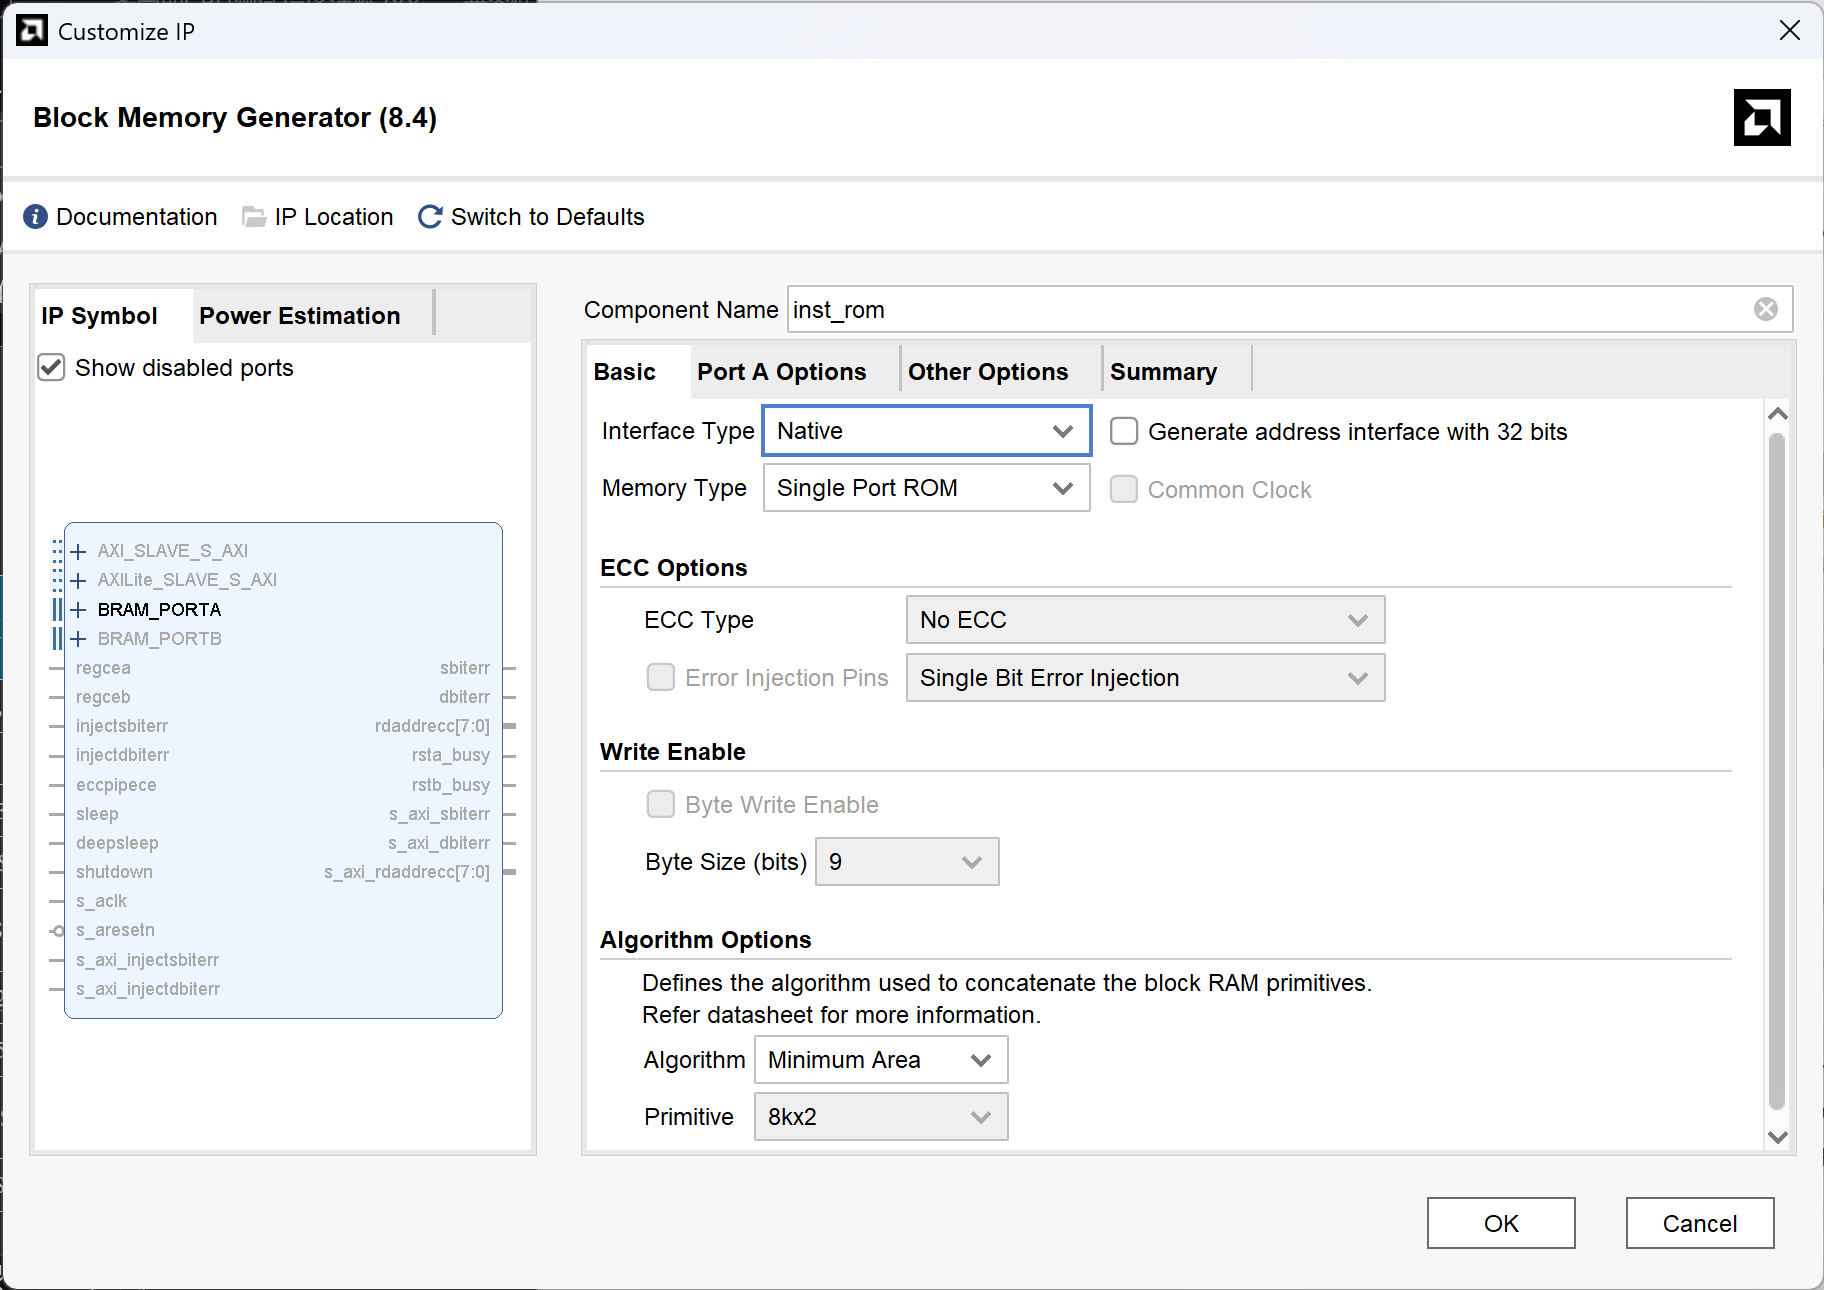
\includegraphics[width=0.5\textwidth]{rom_ip.png}
  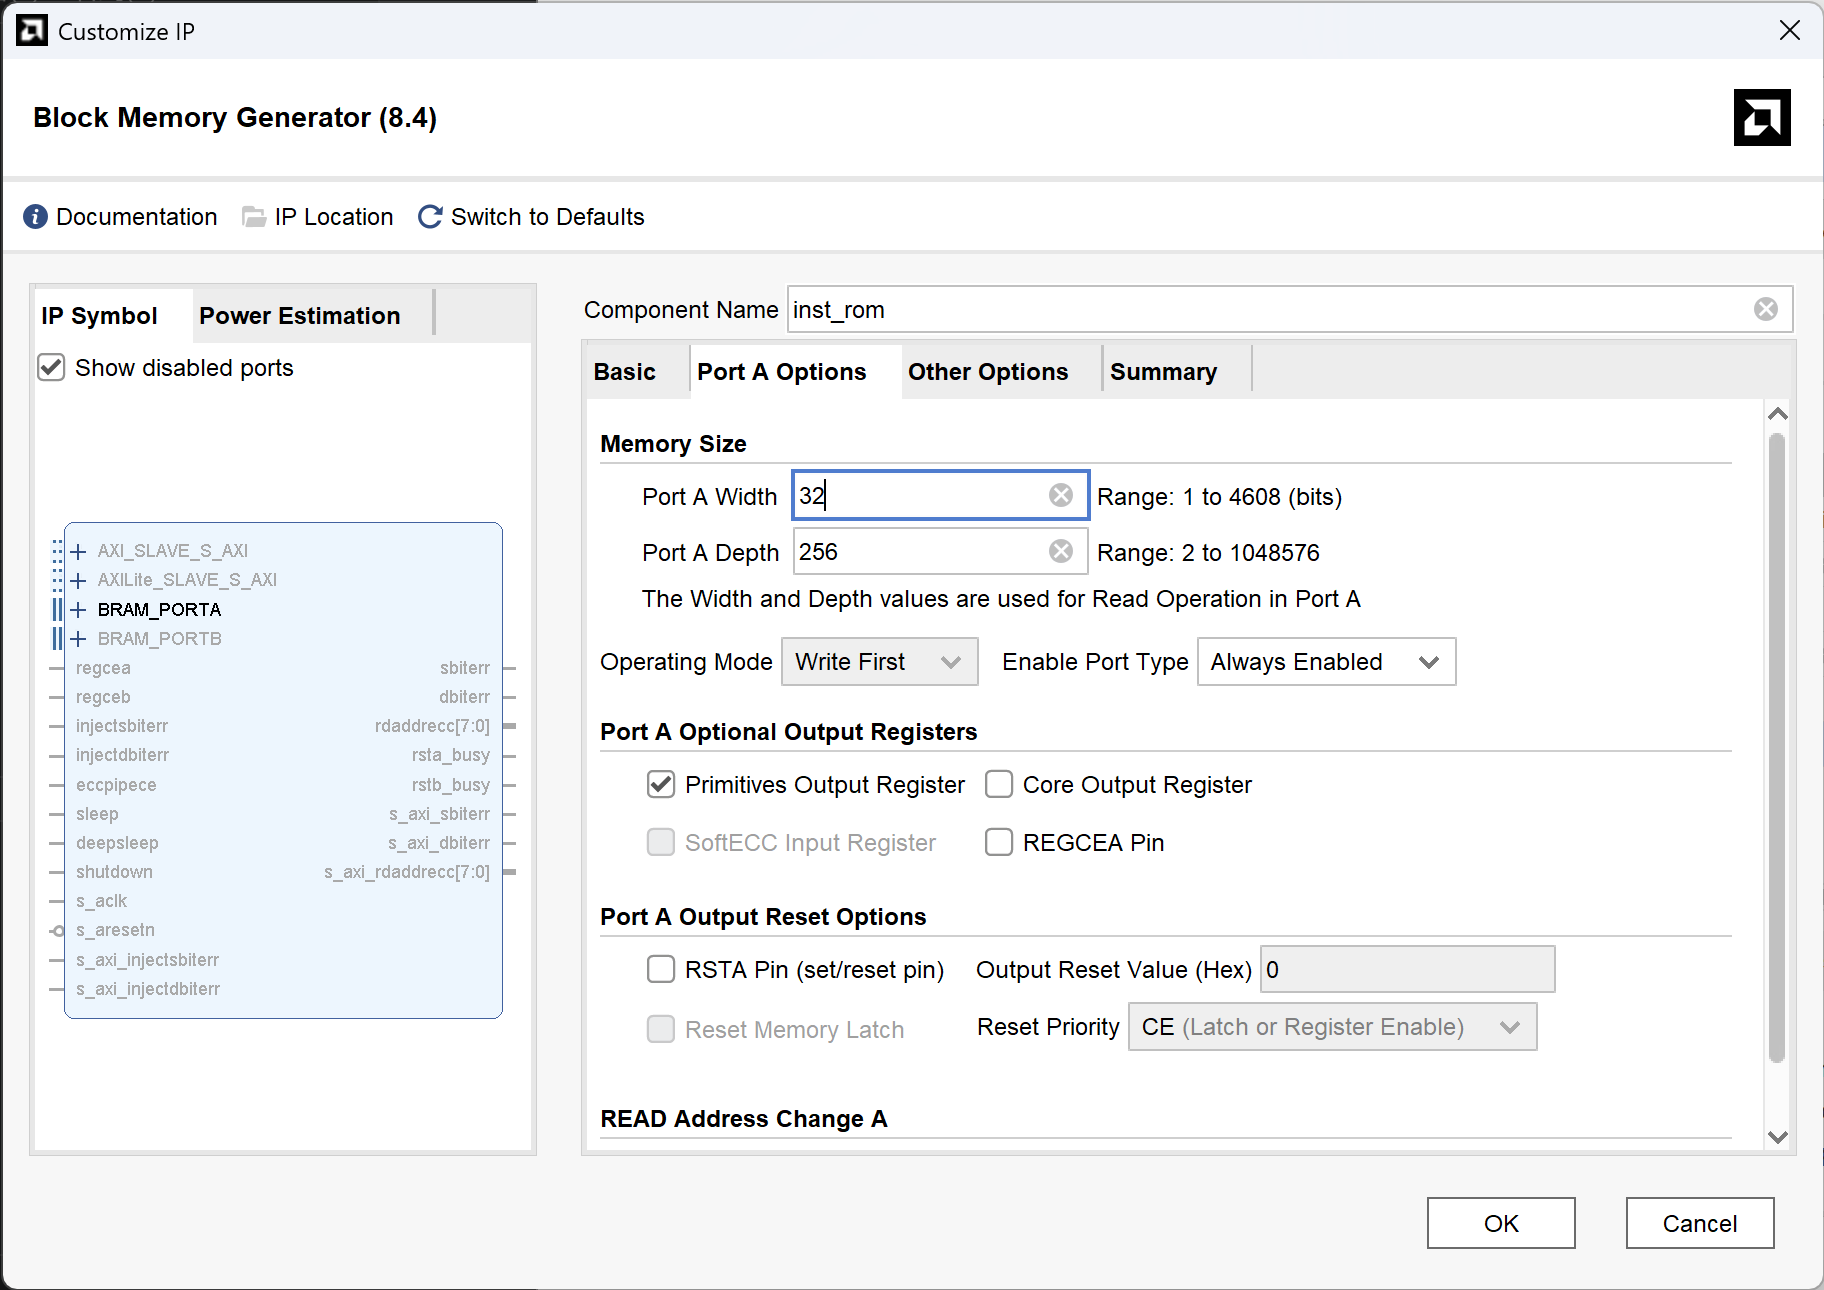
\includegraphics[width=0.5\textwidth]{rom_ip2.png}
  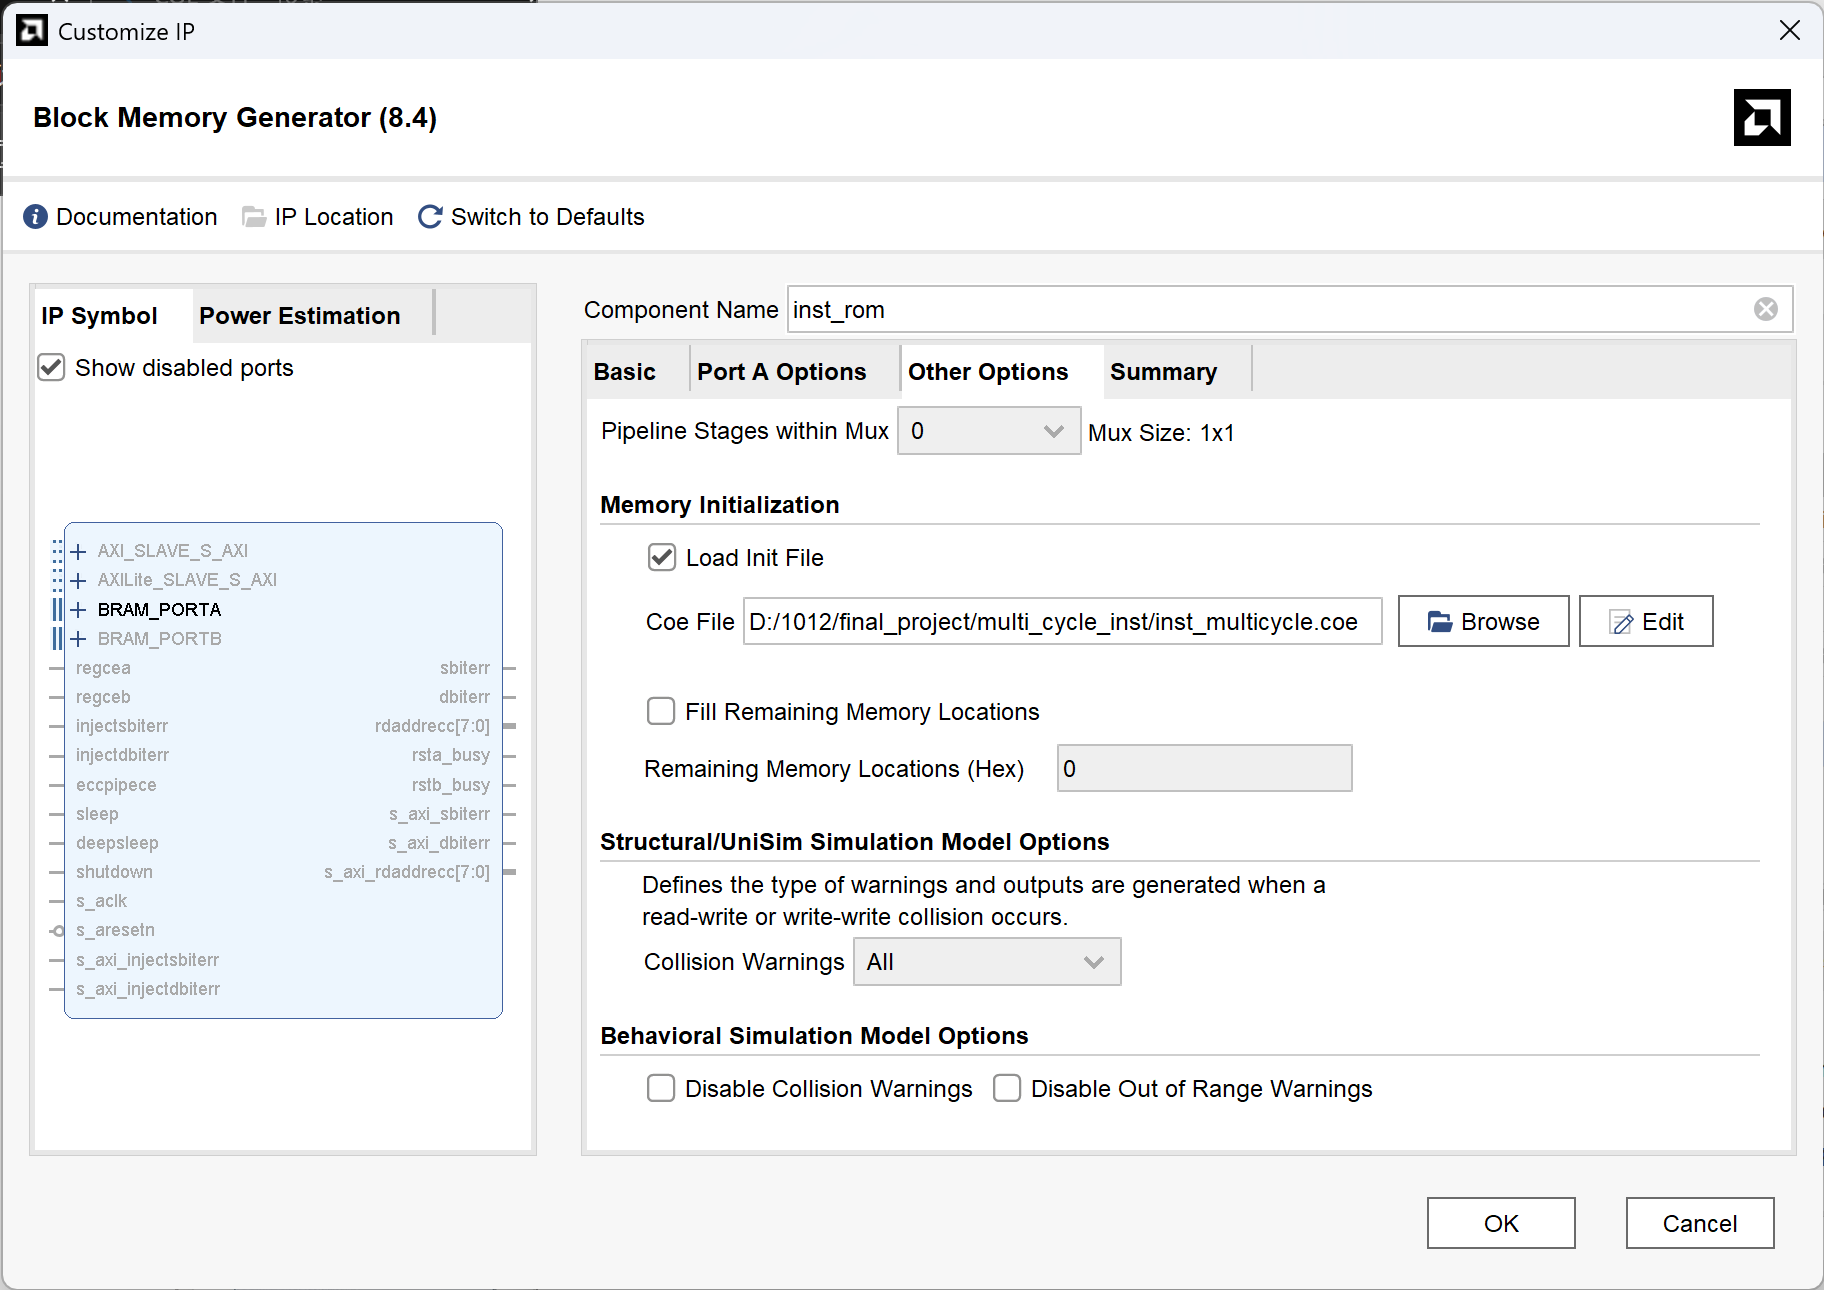
\includegraphics[width=0.5\textwidth]{rom_ip3.png}
  \caption{指令ROM IP核的创建}
\end{figure}

\begin{figure}[h!]
  \centering
  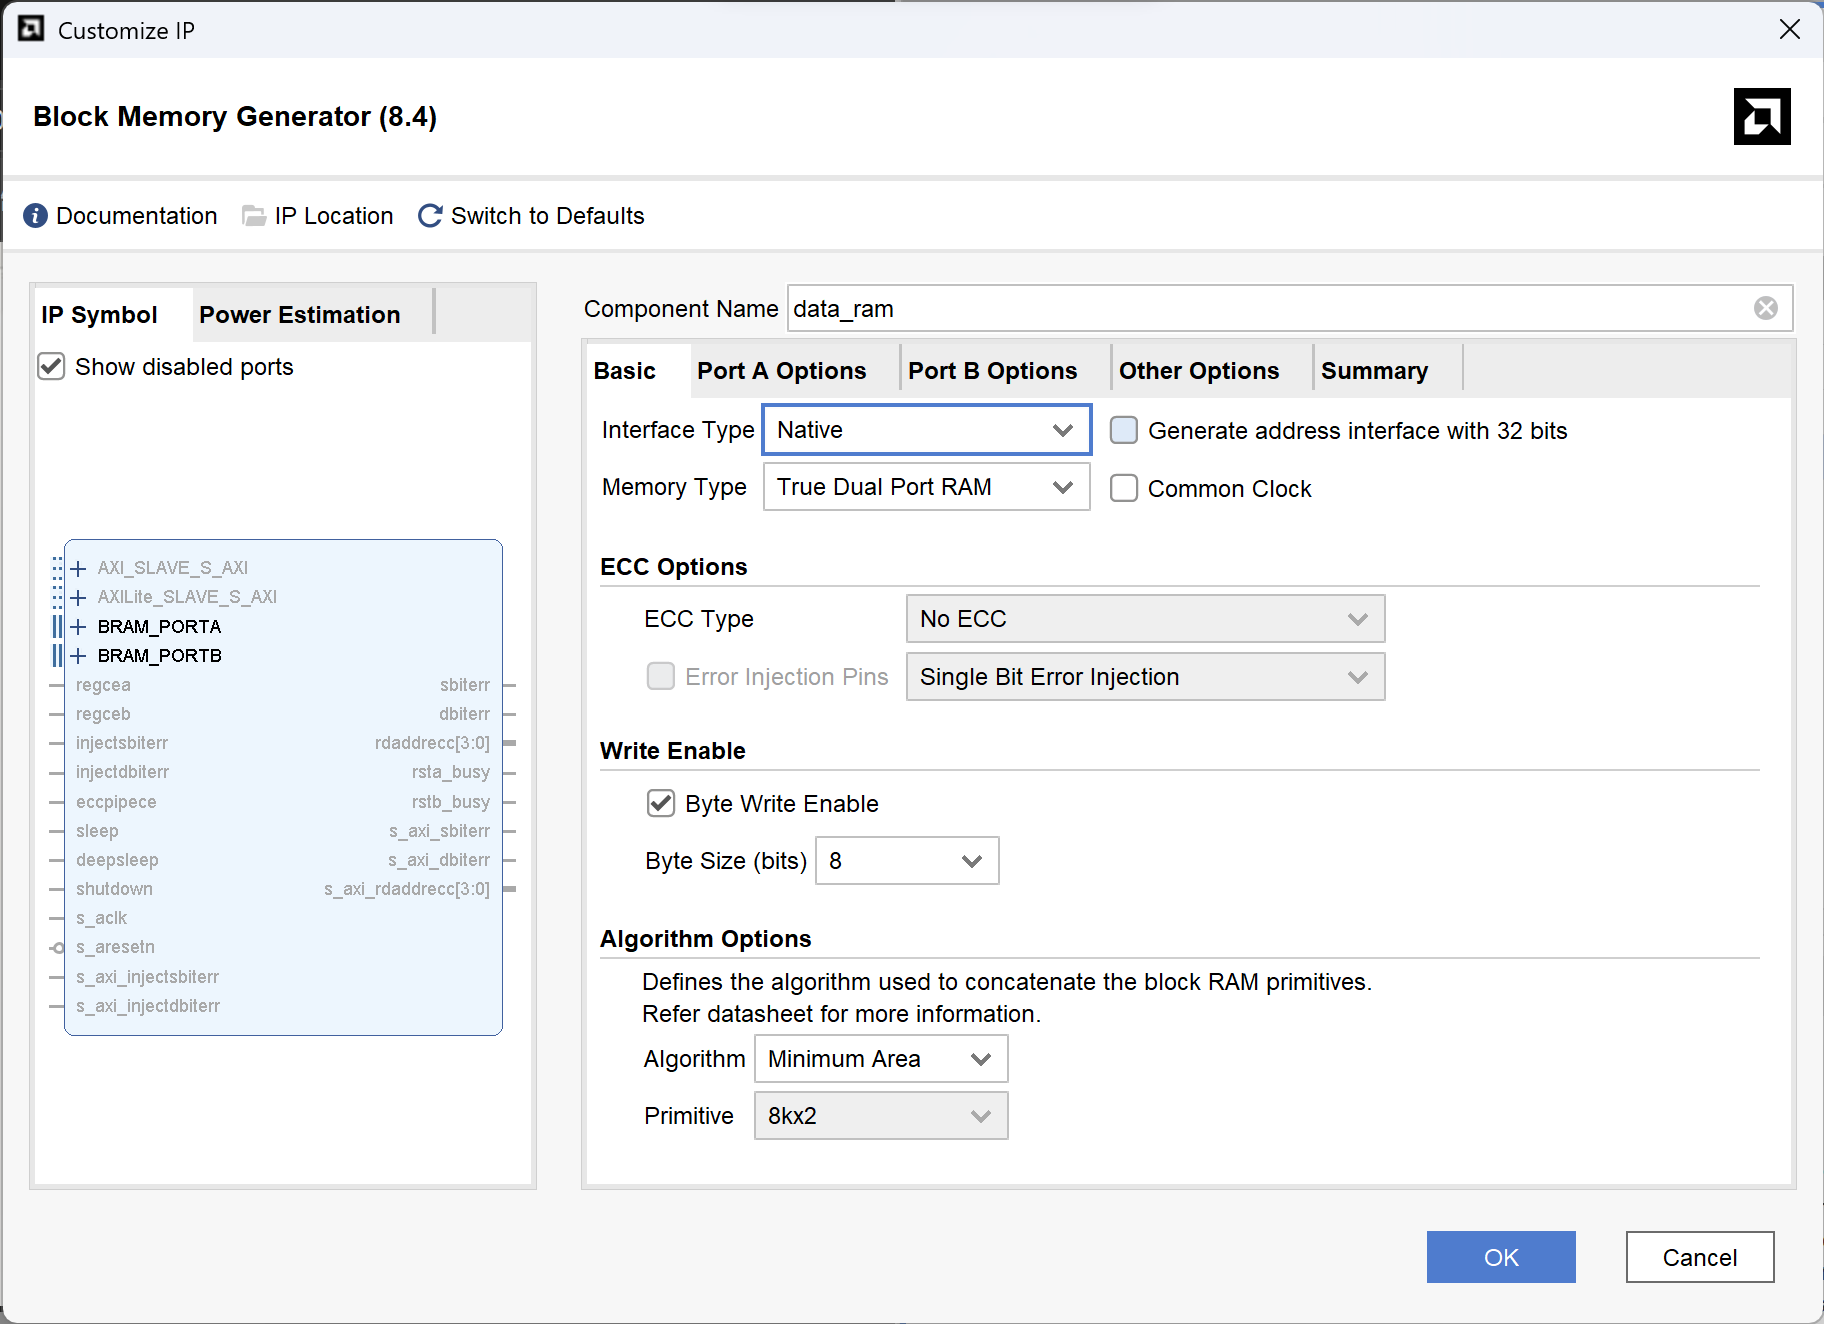
\includegraphics[width=0.5\textwidth]{ram_ip.png}
  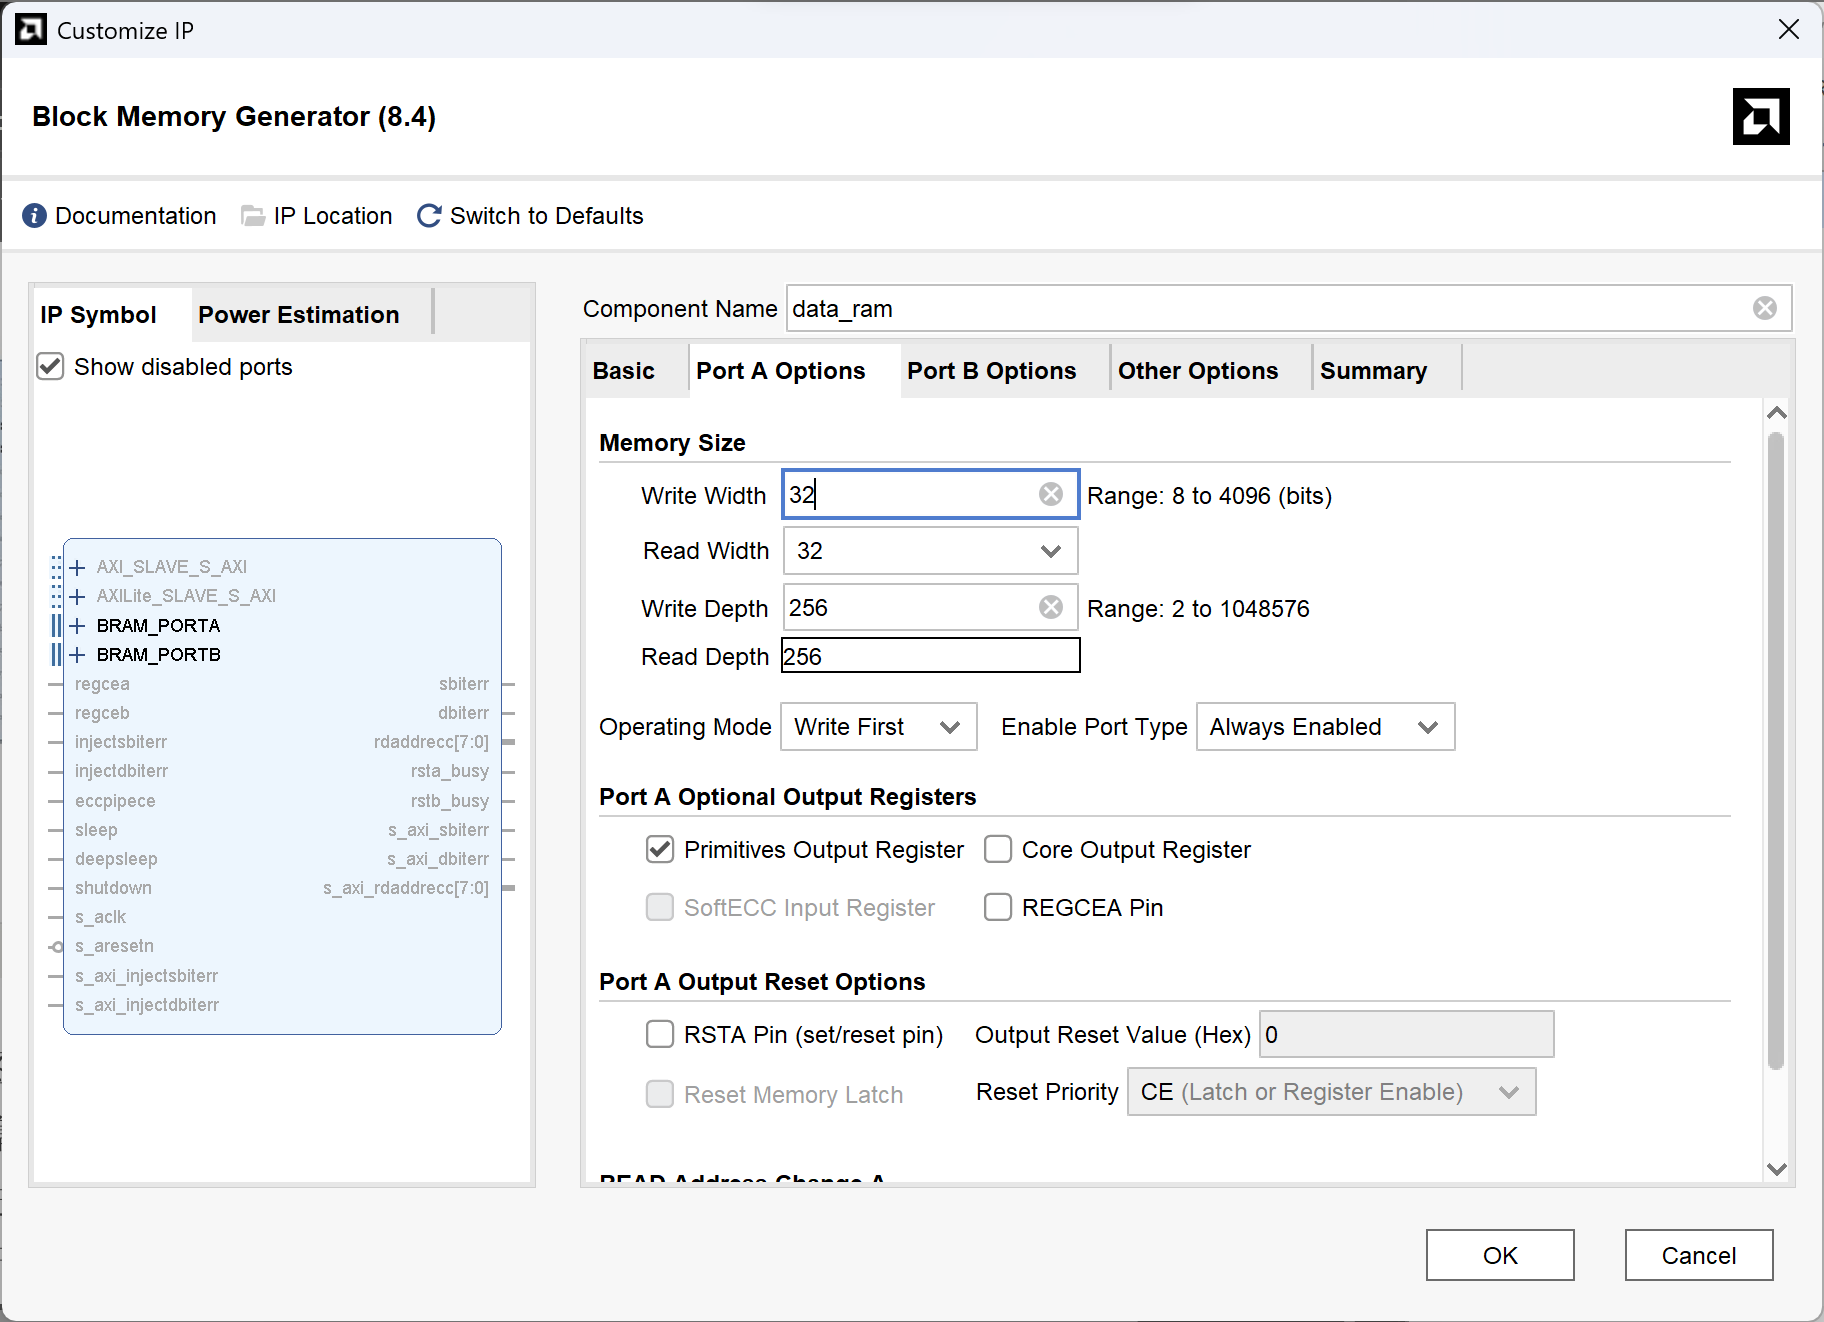
\includegraphics[width=0.5\textwidth]{ram_ip2.png}
  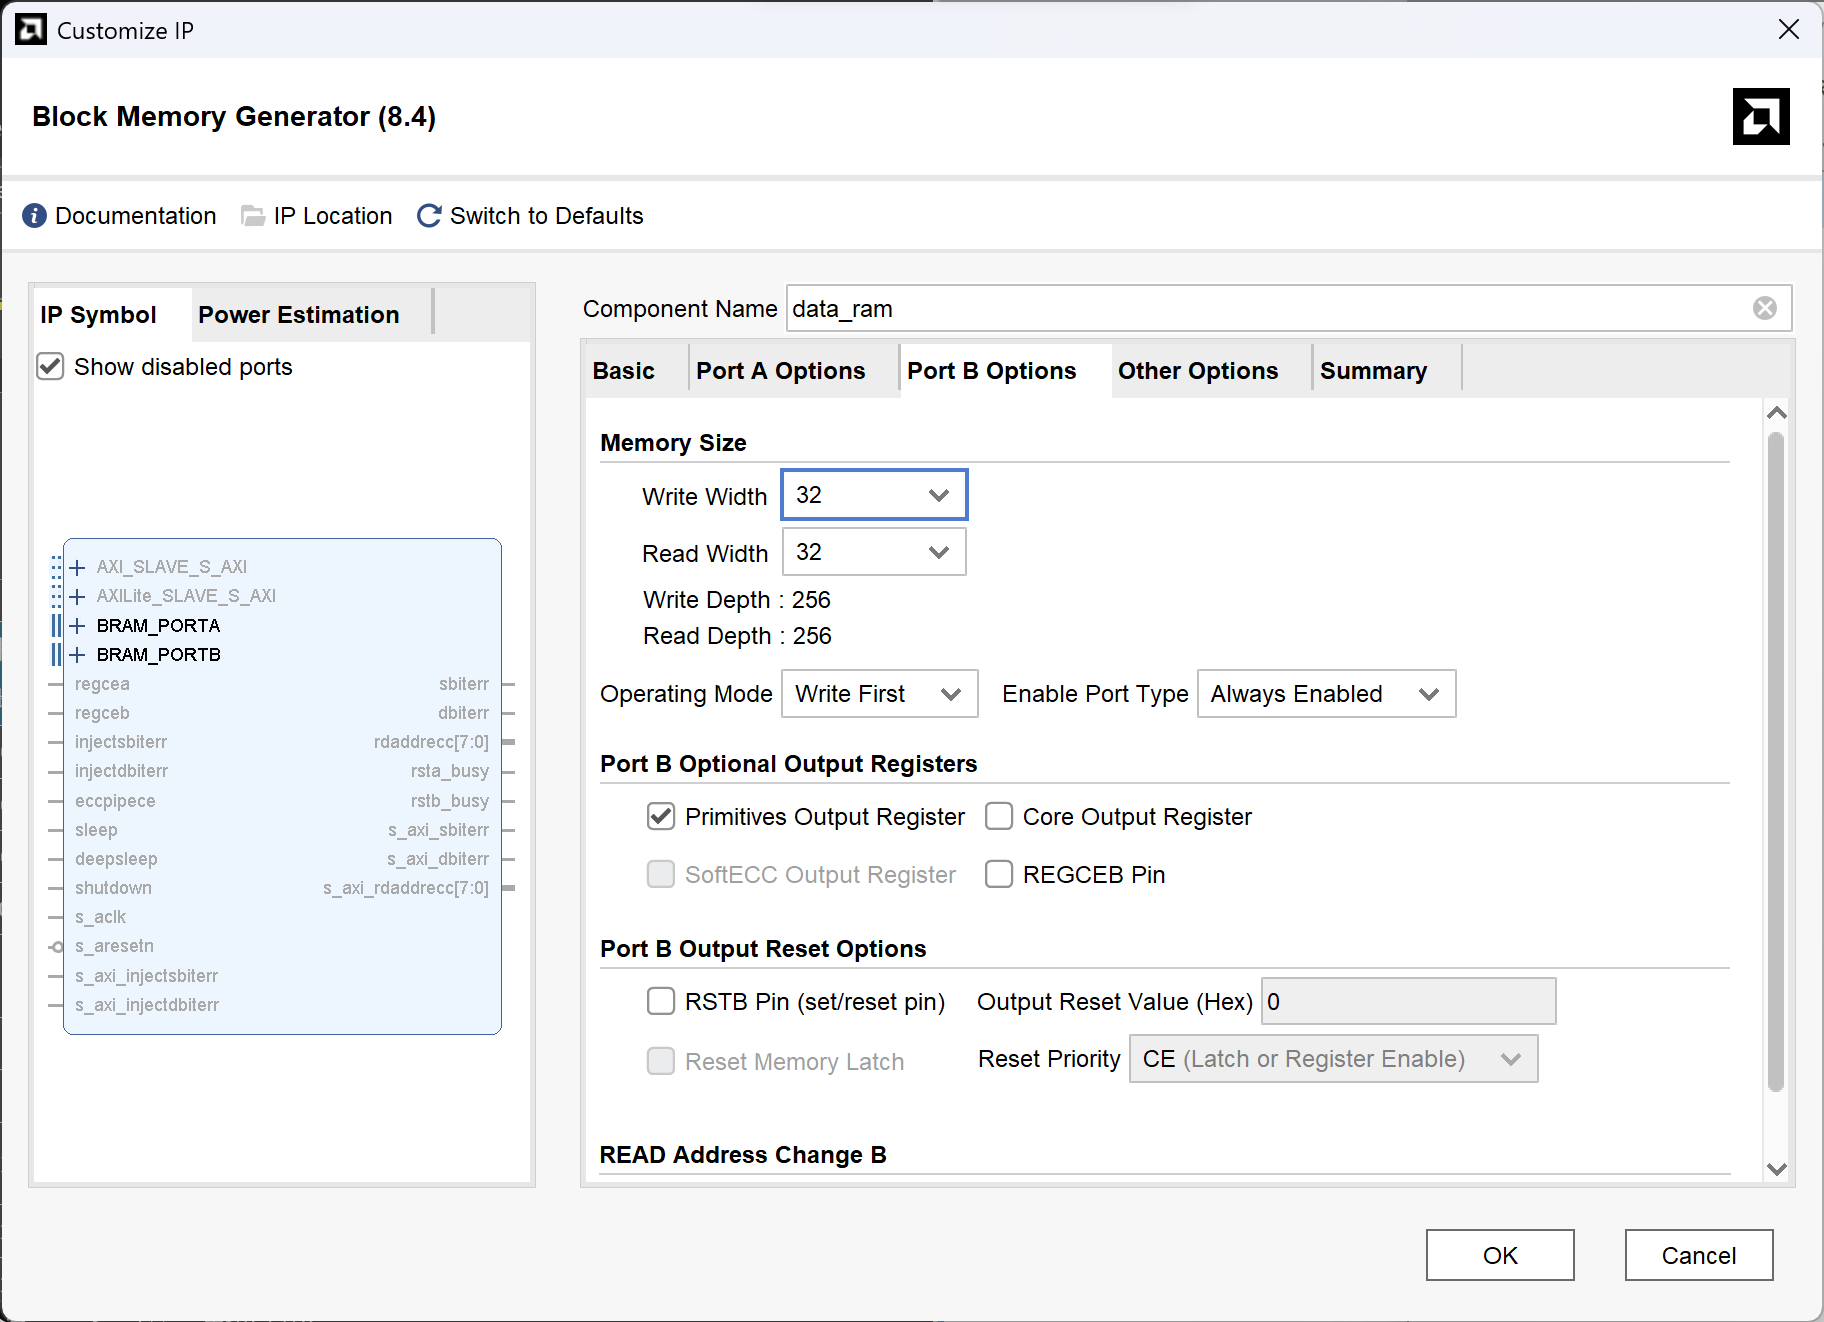
\includegraphics[width=0.5\textwidth]{ram_ip3.png}
  \caption{数据RAM IP核的创建}
\end{figure}

\newpage
\subsection{原始代码的Debug}
通过阅读多周期CPU测试程序的MIPS汇编代码，发现以下问题：
按照标准MIPS实现，
\begin{equation}
  \text{目标地址} = \text{当前指令地址(PC)} + 4 + \text{立即数} \times 4
\end{equation}
但是多周期CPU的实现中是
\begin{equation}
  \text{目标地址} = \text{当前指令地址(PC)} + \text{立即数} \times 4
\end{equation}
\begin{verbatim}
// lab7/decode.v line 181  
assign br_target[31:2] = pc[31:2] + {{14{offset[15]}}, offset};
\end{verbatim}
这与流水线CPU（采用标准实现）不同。
\begin{verbatim}
// lab8/decode.v line 198  
wire [31:0] bd_pc;
assign bd_pc = pc + 3'b100;
// line 225
assign br_target[31:2] = bd_pc[31:2] + {{14{offset[15]}}, offset}; 
// line 272 (延迟槽 PC+8)
assign alu_operand2 = inst_j_link ? 32'd8 :  
                          inst_imm_zero ? {16'd0, imm} :
                          inst_imm_sign ?  {{16{imm[15]}}, imm} : rt_value;
\end{verbatim}
按照标准MIPS，多周期CPU的配套coe文件存在以下异常：

\textbf{1.14H}

\begin{verbatim}
bgez  $25,#16	跳转到54H
\end{verbatim}

此处跳转条件为真的情况下，跳转目标地址应为14+4=18(Hex)=24(Dec), +(16$\times$4)=88(Dec)=58(Hex)
而非54(Hex)。直接跳转到58(Hex)，此时寄存器\$12未正确初始化从而程序会表现异常，
要使程序行为正确，应修改立即数为15。

\textbf{2.30H}

\begin{verbatim}
30H	beq    $8, $3,#2	跳转到38H
\end{verbatim}

同样是一个偏移量计算错误，正确行为：跳转到38H，但立即数为2的情况下，由MIPS分支跳转指令的定义，可知
目标地址变成了(30+4)+(2$\times$4)=3C(Hex)，应修改立即数为1。

\textbf{3.40H}

\begin{verbatim}
40H	bne    $10,$5,#4	跳转到50H
\end{verbatim}

同理，立即数应为3。

\textbf{4.88H}

\begin{verbatim}
88H	bltz    $16, #6	跳转到A0H
\end{verbatim}

同理，立即数应为5。

\textbf{5.90H}

\begin{verbatim}
90H	bne   $28,$29,#7	不跳转/跳转ACH
\end{verbatim}

要跳转到AC(Hex)=172(Dec)，偏移量应为(172-(9$\times$16)-4)/4=6(Dec)。
立即数应为6。

\subsection{五级流水线CPU的改进：旁路}
本次最终实现没有改动原有的延迟槽机制，也没有改动\texttt{jal/jalr}写回
\texttt{PC+8}的语义，而是在此基础上把原本“只要相关就统一停顿”的策略改成了
“EXE级优先前递，只有确实无法前递时再停顿”。也就是说，当前流水线并不是一个
“所有相关都能零开销解决”的理想模型，而是一种“EXE级前递 + 必要停顿 + ID级分支保守处理”
的混合实现：能在后续流水级中拿到稳定结果时，就尽量旁路到消费者；只有结果尚未准备好，
或者该类指令必须在ID级立即得到操作数时，才主动阻塞流水线。

前递相关的元信息主要在\texttt{pipeline\_cpu.v}中整理。设计中从
\texttt{ID\_EXE\_bus\_r}与\texttt{EXE\_MEM\_bus\_r}中拆出目的寄存器号、
寄存器写使能以及结果类型，并据此构造两类控制信号。第一类是
\texttt{EXE\_slow\_result}和\texttt{MEM\_slow\_result}，用于标记当前阶段结果
虽然最终会写回寄存器，但此时还不能安全地被后继指令直接使用；在本实现中，
\texttt{load}、\texttt{mfhi}、\texttt{mflo}、\texttt{mfc0}都被归入这一类慢结果。
第二类是可直接用于前递的旁路信息，即\texttt{MEM\_fwd\_wen}、
\texttt{MEM\_fwd\_wdest}和\texttt{MEM\_fwd\_data}，它们构成了从MEM侧送往消费者EXE级的
第一路前递源；WB级则直接复用\texttt{rf\_wen}、\texttt{rf\_wdest}和\texttt{rf\_wdata}
作为第二路前递源。这样做的含义是：并不是所有结果都能从MEM侧旁路，只有已经形成稳定整数结果的
普通ALU类写回，才被作为快速前递对象处理。

冲突检测逻辑位于\texttt{decode.v}。这里首先区分了两类指令：一类是在ID级就必须立刻使用源寄存器值的
控制转移指令，例如\texttt{jr}、\texttt{jalr}、\texttt{beq}、\texttt{bne}、
\texttt{bgez}、\texttt{bgtz}、\texttt{blez}和\texttt{bltz}；另一类是直到进入EXE级才真正消费
源操作数的指令，例如普通算术逻辑运算、访存地址计算以及\texttt{store}写数据准备。对于前一类指令，
只要它们依赖的寄存器正由EXE、MEM或WB中的更早指令准备写回，就采用保守停顿策略；这也说明当前实现
\textbf{没有加入ID级分支旁路}，因此分支相关仍通过等待来保证正确性。对于后一类指令，则不再因为
“存在相关”就一律阻塞，而是只在依赖项属于慢结果时停顿，也就是典型的\texttt{load-use}相关以及
\texttt{mfhi/mflo/mfc0}等特殊结果相关。

真正的数据选择发生在\texttt{exe.v}。EXE级会分别比较当前指令的\texttt{rs}和\texttt{rt}与
\texttt{MEM\_fwd\_wdest}、\texttt{WB\_fwd\_wdest}是否匹配；若命中MEM前递源，则优先选用
\texttt{MEM\_fwd\_data}；若MEM未命中但WB命中，则退而选用\texttt{WB\_fwd\_data}；只有两级都未命中时，
才回退到寄存器堆读出的原始值。这套选择逻辑同时服务于\texttt{alu\_operand1}、
\texttt{alu\_operand2}和\texttt{store\_data}。特别是\texttt{store\_data}最终直接取自已经完成
旁路选择后的\texttt{rt\_value}，因此本次实现不仅支持普通的\texttt{ALU $\rightarrow$ ALU}前递，
也支持\texttt{ALU $\rightarrow$ store}前递，而不是只解决算术指令之间的相关。

\begin{itemize}
  \item 已支持的主要场景包括：\texttt{ALU $\rightarrow$ ALU}、跨1条指令的\texttt{ALU $\rightarrow$ ALU}、\texttt{ALU $\rightarrow$ store}。
  \item 仍需停顿的场景包括：\texttt{load-use}、ID级分支/\texttt{jr}/\texttt{jalr}相关、\texttt{mfhi/mflo/mfc0}等慢结果相关。
  \item 乘法仍按原多周期乘法部件的完成时刻决定\texttt{EXE\_over}，它不属于“单拍即可直接旁路”的普通ALU结果。
\end{itemize}

上述改进的直接效果是：普通整数运算之间不再需要大量人为插入\texttt{nop}，\texttt{store}指令也可以
直接使用前面刚算出的结果；与此同时，控制相关和慢结果相关仍保留必要停顿。这样既保留了原有流水线控制模型、
延迟槽语义和异常处理路径，又显著减少了不必要的流水线空转。

\subsection{多周期CPU向标准MIPS分支语义的修正}
为保证多周期CPU与标准MIPS定义一致，最终版本直接修改了\texttt{lab7}硬件，
将分支目标地址计算改为
\begin{equation}
  \text{BranchTarget} = PC + 4 + (\text{offset} \ll 2)
\end{equation}
因此，\texttt{inst\_multicycle.coe}中对应的5处分支立即数也同步修正。
这样处理后，多周期CPU和五级流水线CPU对分支偏移量的解释重新一致，
后续调试与验证不再需要额外区分“非标准多周期版本”和“标准流水线版本”。

\subsection{多周期CPU的复现}
\begin{figure}[h!]
  \centering
  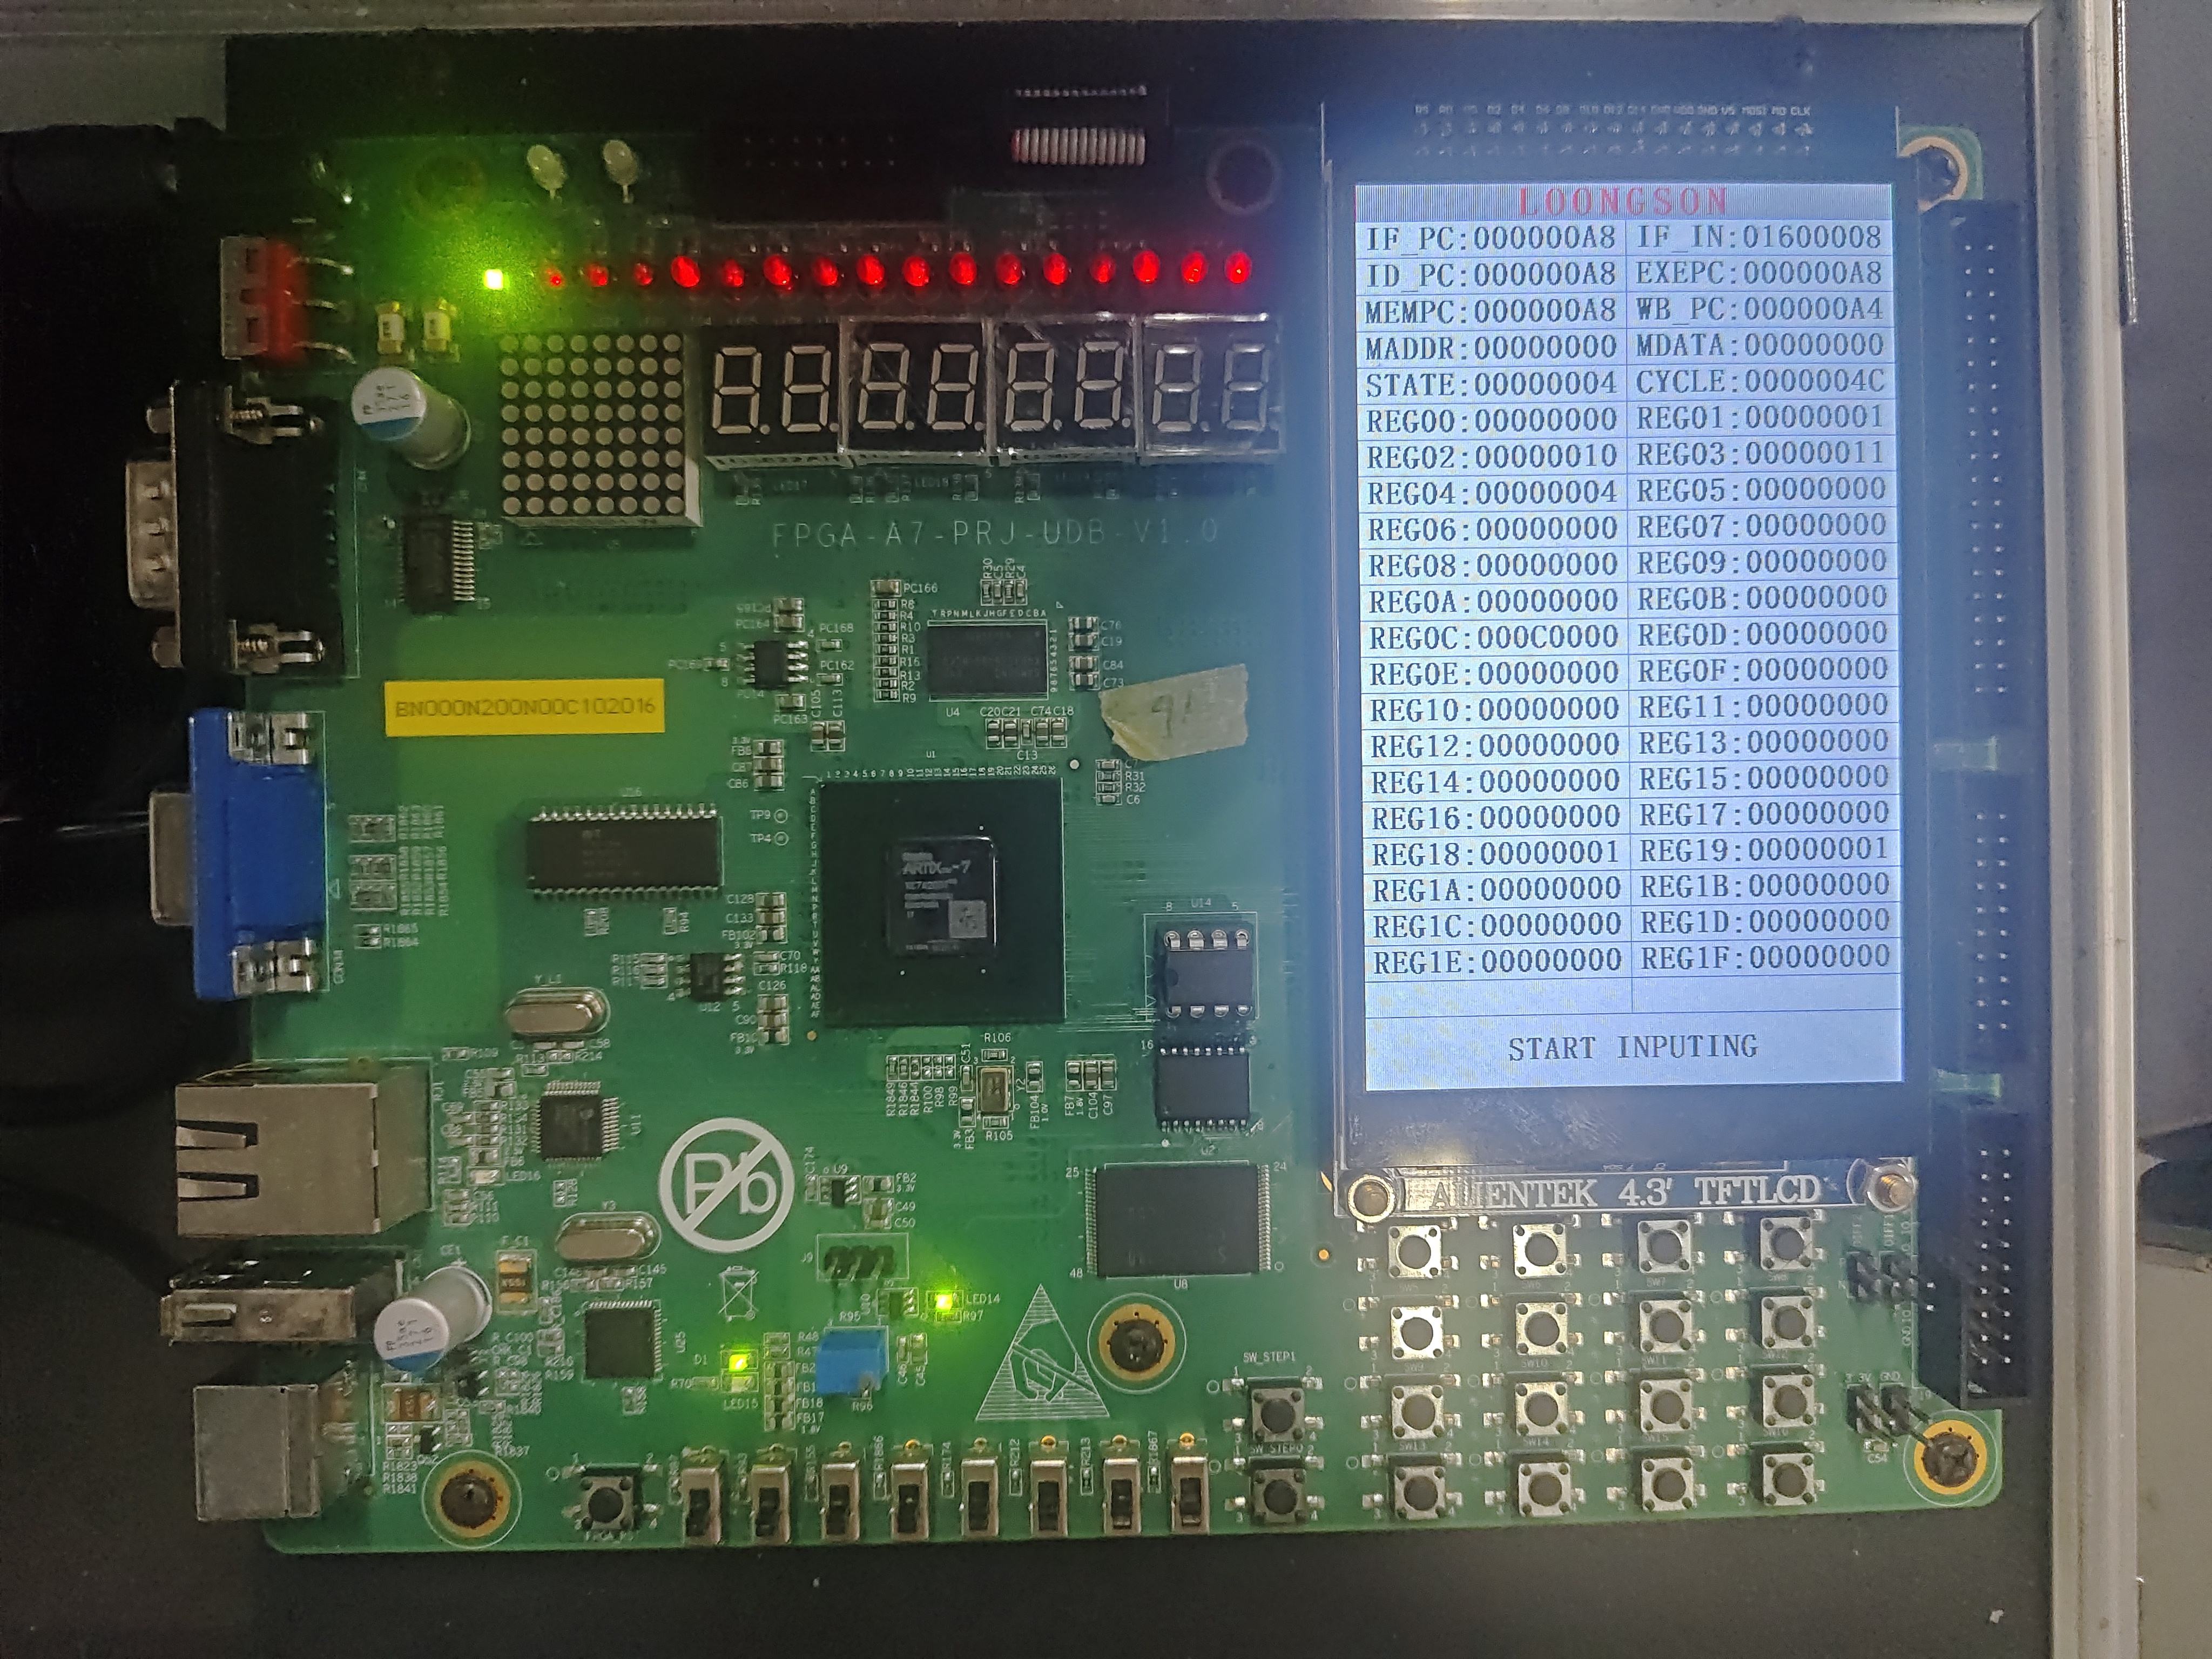
\includegraphics[width=\textwidth]{multi_re.jpg}
  \caption{多周期CPU的复现}
\end{figure}

\subsection{流水线CPU的复现}
\begin{figure}[h!]
  \centering
  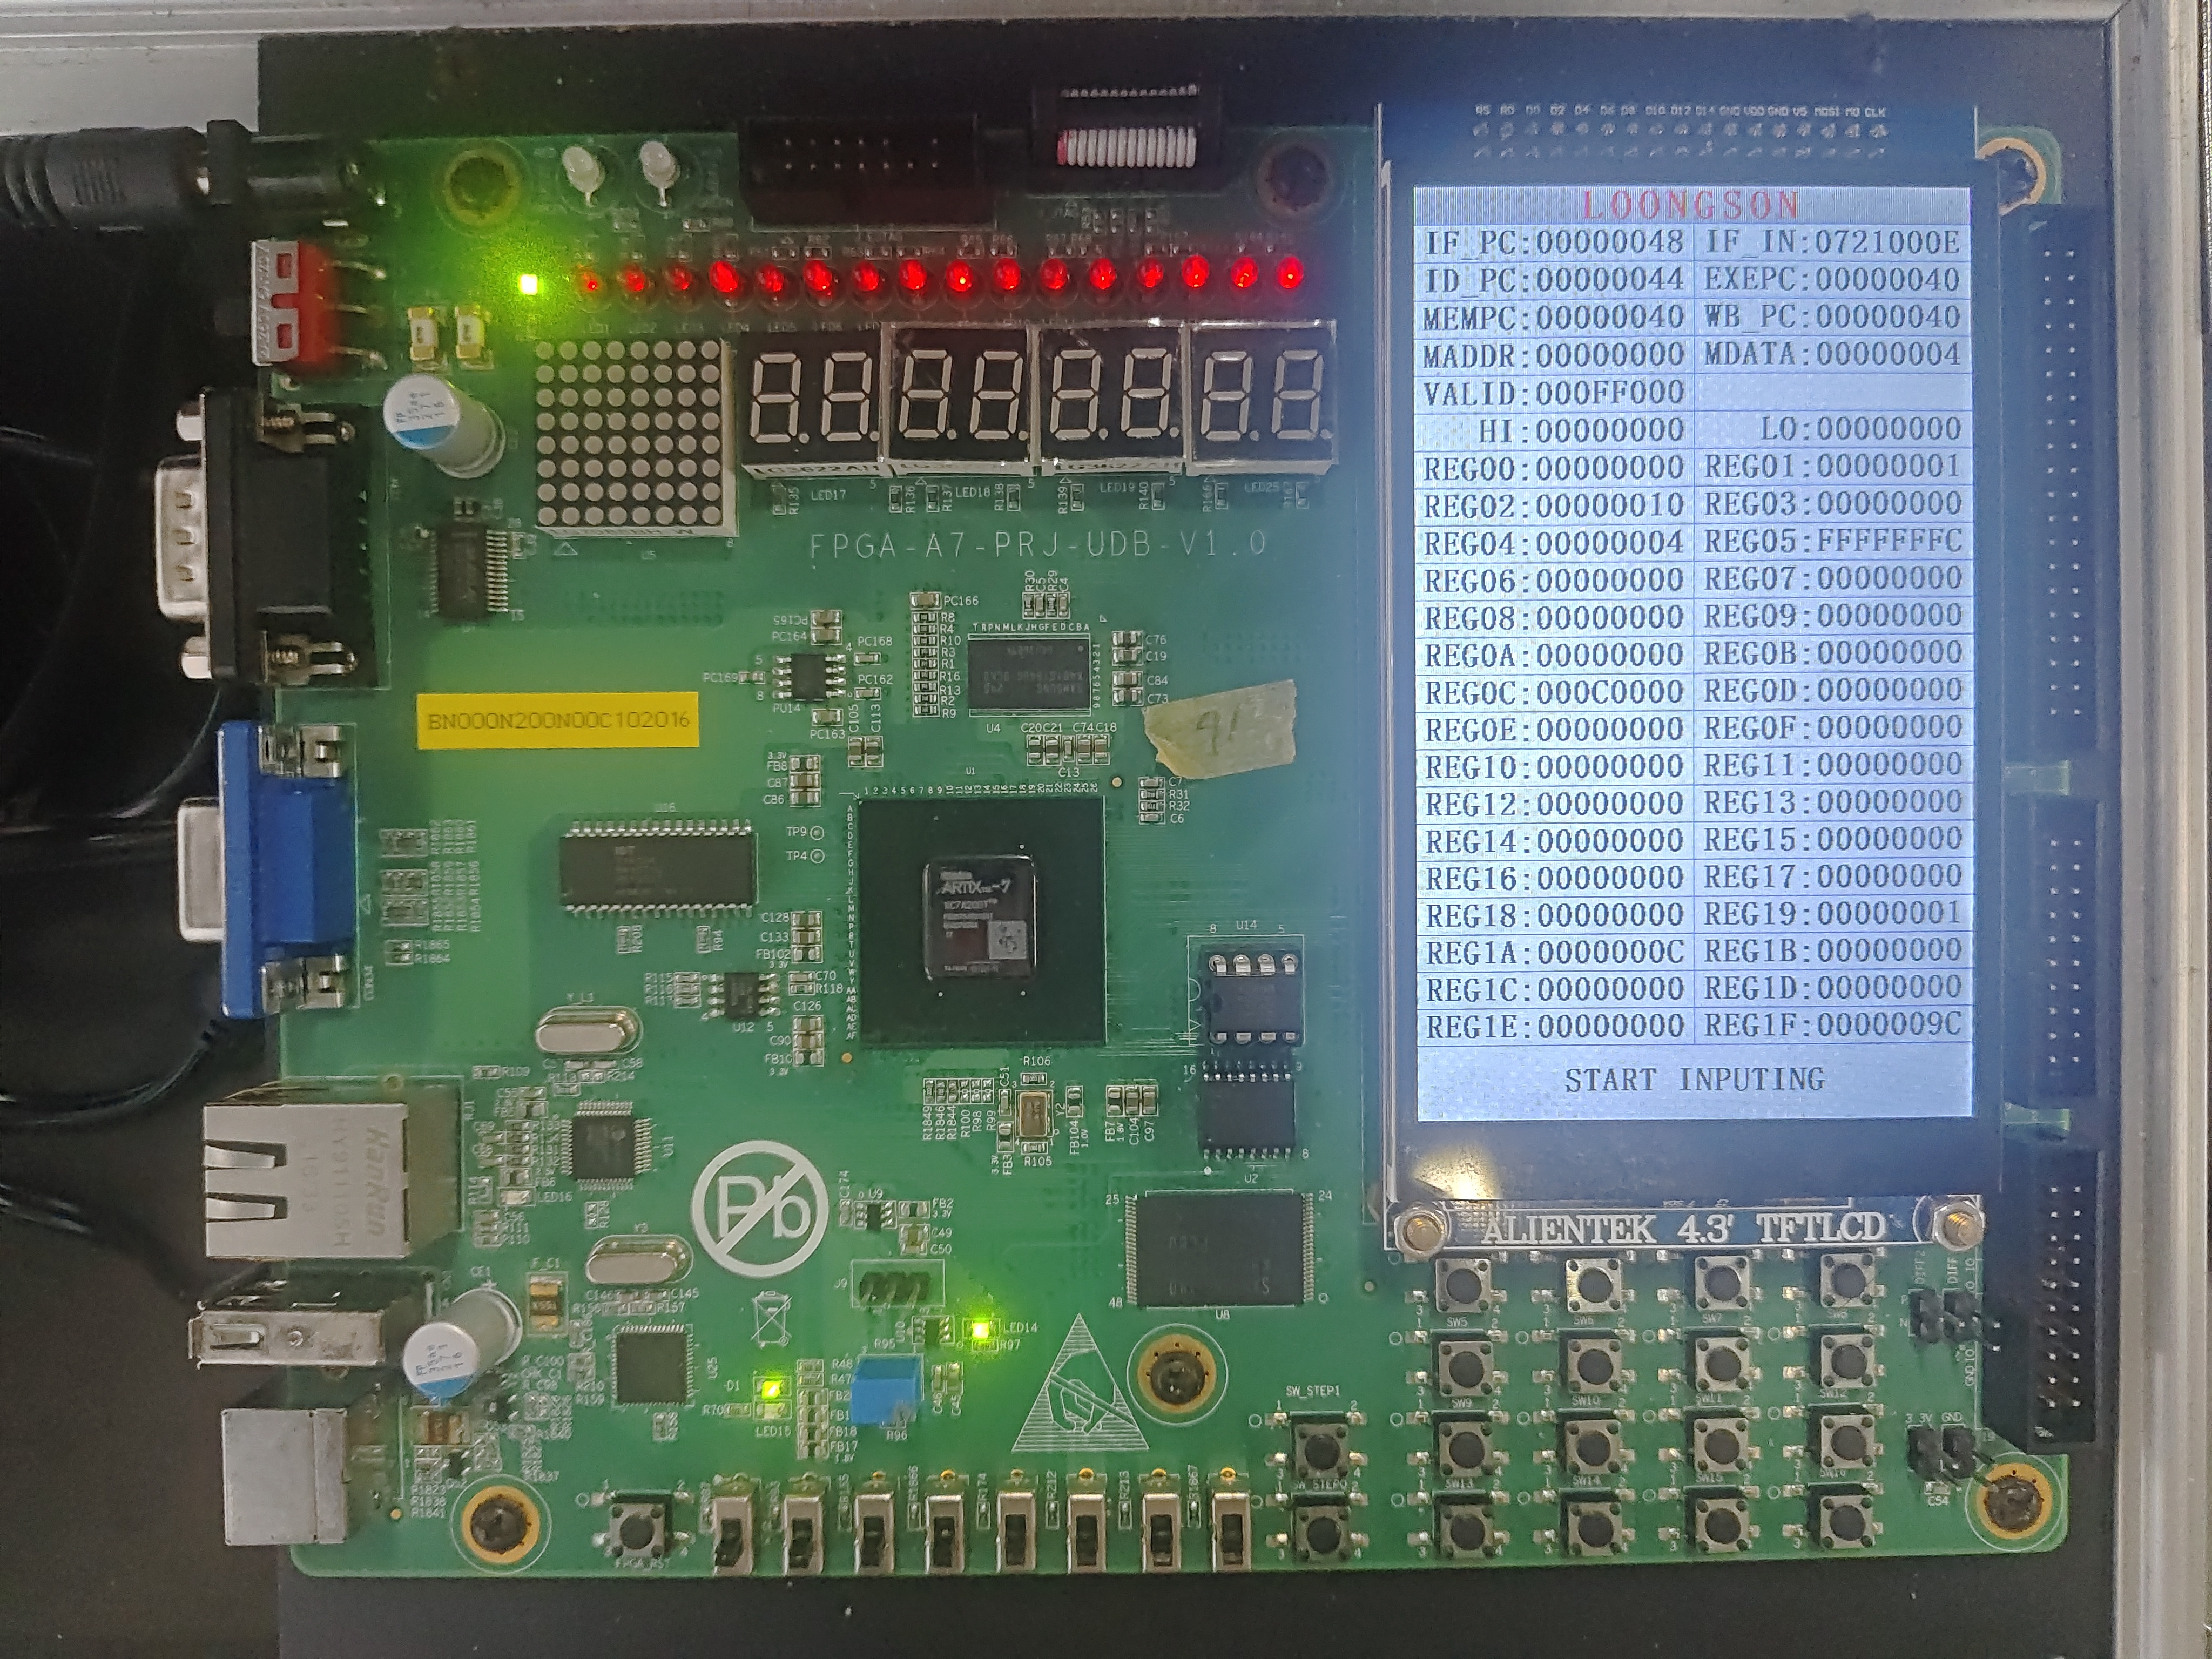
\includegraphics[width=\textwidth]{pipeline_re.jpg}
  \caption{流水线CPU的复现}
\end{figure}

\newpage


\section{关键代码}
\subsection{多周期CPU分支基址修复}
\begin{verbatim}
// final_project/lab7/.../decode.v
assign br_target[31:2] = pc[31:2] + 30'd1
                       + {{14{offset[15]}}, offset};
\end{verbatim}

\subsection{流水线CPU由“ID级统一停顿”改为“EXE级前递+必要停顿”}
\begin{verbatim}
// final_project/lab8/.../pipeline_cpu.v
assign EXE_slow_result = EXE_valid & EXE_meta_rf_wen
                       & (EXE_meta_mem_control[3] | EXE_meta_mfhi
                       |  EXE_meta_mflo | EXE_meta_mfc0);
assign MEM_fwd_wen     = MEM_valid & MEM_meta_rf_wen
                       & ~(MEM_meta_mem_control[3] | MEM_meta_mfhi
                       |   MEM_meta_mflo | MEM_meta_mfc0);
\end{verbatim}

\begin{verbatim}
// final_project/lab8/.../decode.v
assign rs_wait_id  = rs_read_id & (exe_dep_rs | mem_dep_rs | wb_dep_rs);
assign rt_wait_id  = rt_read_id & (exe_dep_rt | mem_dep_rt | wb_dep_rt);
assign rs_wait_exe = rs_read_exe
                   & ((exe_dep_rs & EXE_slow_result)
                   |  (mem_dep_rs & MEM_slow_result));
assign rt_wait_exe = rt_read_exe
                   & ((exe_dep_rt & EXE_slow_result)
                   |  (mem_dep_rt & MEM_slow_result));
\end{verbatim}

\begin{verbatim}
// final_project/lab8/.../exe.v
assign rs_value = rs_from_mem ? MEM_fwd_data :
                  rs_from_wb  ? WB_fwd_data  : rs_raw_value;
assign rt_value = rt_from_mem ? MEM_fwd_data :
                  rt_from_wb  ? WB_fwd_data  : rt_raw_value;
\end{verbatim}

\begin{verbatim}
// final_project/lab8/.../exe.v
assign store_data = rt_value;
\end{verbatim}
上述修改的效果是：
\begin{itemize}
  \item 普通ALU结果可以从MEM/WB直接前递到消费者指令所在的EXE级；
  \item store的数据也可以前递，不再要求前面必须插入大量\texttt{nop}；
  \item 分支、\texttt{jr/jalr}仍保持保守策略，在ID级等待源寄存器值真正可见，而不是在ID级做旁路；
  \item \texttt{load/mfhi/mflo/mfc0}这类结果继续视为“慢结果”，只在必要时停顿。
\end{itemize}

\section{计算任务：斐波那契数列特定项的计算}
计算任务最终采用和单周期CPU实验中固定输入的迭代版\texttt{Fib(10)}程序，
源码单独保存在\texttt{final\_project/pipeline\_inst/fib10\_pipeline.asm}中。
考虑到流水线CPU复位入口地址固定为\texttt{34H}，新的\texttt{inst\_pipeline.coe}
前部保留了\texttt{00H\textasciitilde30H}的填充区，使程序从\texttt{34H}开始执行。

在多周期和流水线版本的实现中，均统计完成斐波那契数列第10项所耗费的时钟周期数并加以显示。

程序的核心循环如下：
\begin{verbatim}
addiu $11, $0, 9       # remaining iterations
loop:
  addiu $11, $11, -1
  addu  $12, $9,  $10
  addu  $13, $12, $0
  addu  $9,  $10, $0
  addu  $10, $12, $0
  bgtz  $11, loop
  addu  $14, $10, $0   # delay slot
\end{verbatim}
该版本主要覆盖了以下相关场景：
\begin{itemize}
  \item \texttt{addu \$12,\$9,\$10 -> addu \$13,\$12,\$0}：ALU$\rightarrow$ALU前递；
  \item \texttt{addu \$12,\$9,\$10 -> addu \$10,\$12,\$0}：跨1条指令的ALU前递；
  \item \texttt{addu \$14,\$10,\$0 -> sw \$14,4(\$0)}：ALU$\rightarrow$store前递；
  \item \texttt{bgtz}保留原有延迟槽，末尾进入稳定自循环，便于仿真和上板观察。
\end{itemize}

\subsection{验证结果}
\subsection{多周期CPU上的斐波那契计算程序}
\begin{verbatim}
Mem[1] = 0x00000037
$10 = 0x00000037
fib_done = 1
cycle_count = 273
\end{verbatim}

\subsubsection{原多周期测试程序}
完成本地仿真。
修复后的多周期程序能够沿预期路径继续执行，仿真末期观测到：
\begin{verbatim}
PC      = 0x00000080
GPR[12] = 0x000C0000
Mem[5]  = 0x000C000D   // 对应字节地址 0x14
Mem[7]  = 0x00000011   // 对应字节地址 0x1C
\end{verbatim}
这说明修复后的CPU与修正后的\texttt{inst\_multicycle.coe}能够正确配合工作。

\subsubsection{原流水线测试程序}
原始测试程序被保留为\texttt{inst\_pipeline\_regression.coe}。
为验证前递改动没有破坏原有功能，对该程序临时转换出的MIF做了同样的行为级仿真，
在仿真末期观测到如下稳定状态：
\begin{verbatim}
IF_pc = 0x00000030
WB_pc = 0x00000030
HI    = 0x00000050
LO    = 0x0000000C
Mem[0]= 0x00000008
Mem[1]= 0x00000010
Mem[2]= 0x00000011
Mem[3]= 0x00000004
Mem[4]= 0x0000000D
\end{verbatim}
说明原有包含乘法、HI/LO、CP0与异常相关路径的程序没有因为本次前递改造而失效。

\newpage
\subsubsection{上板验证}
\begin{figure}[h!]
  \centering
  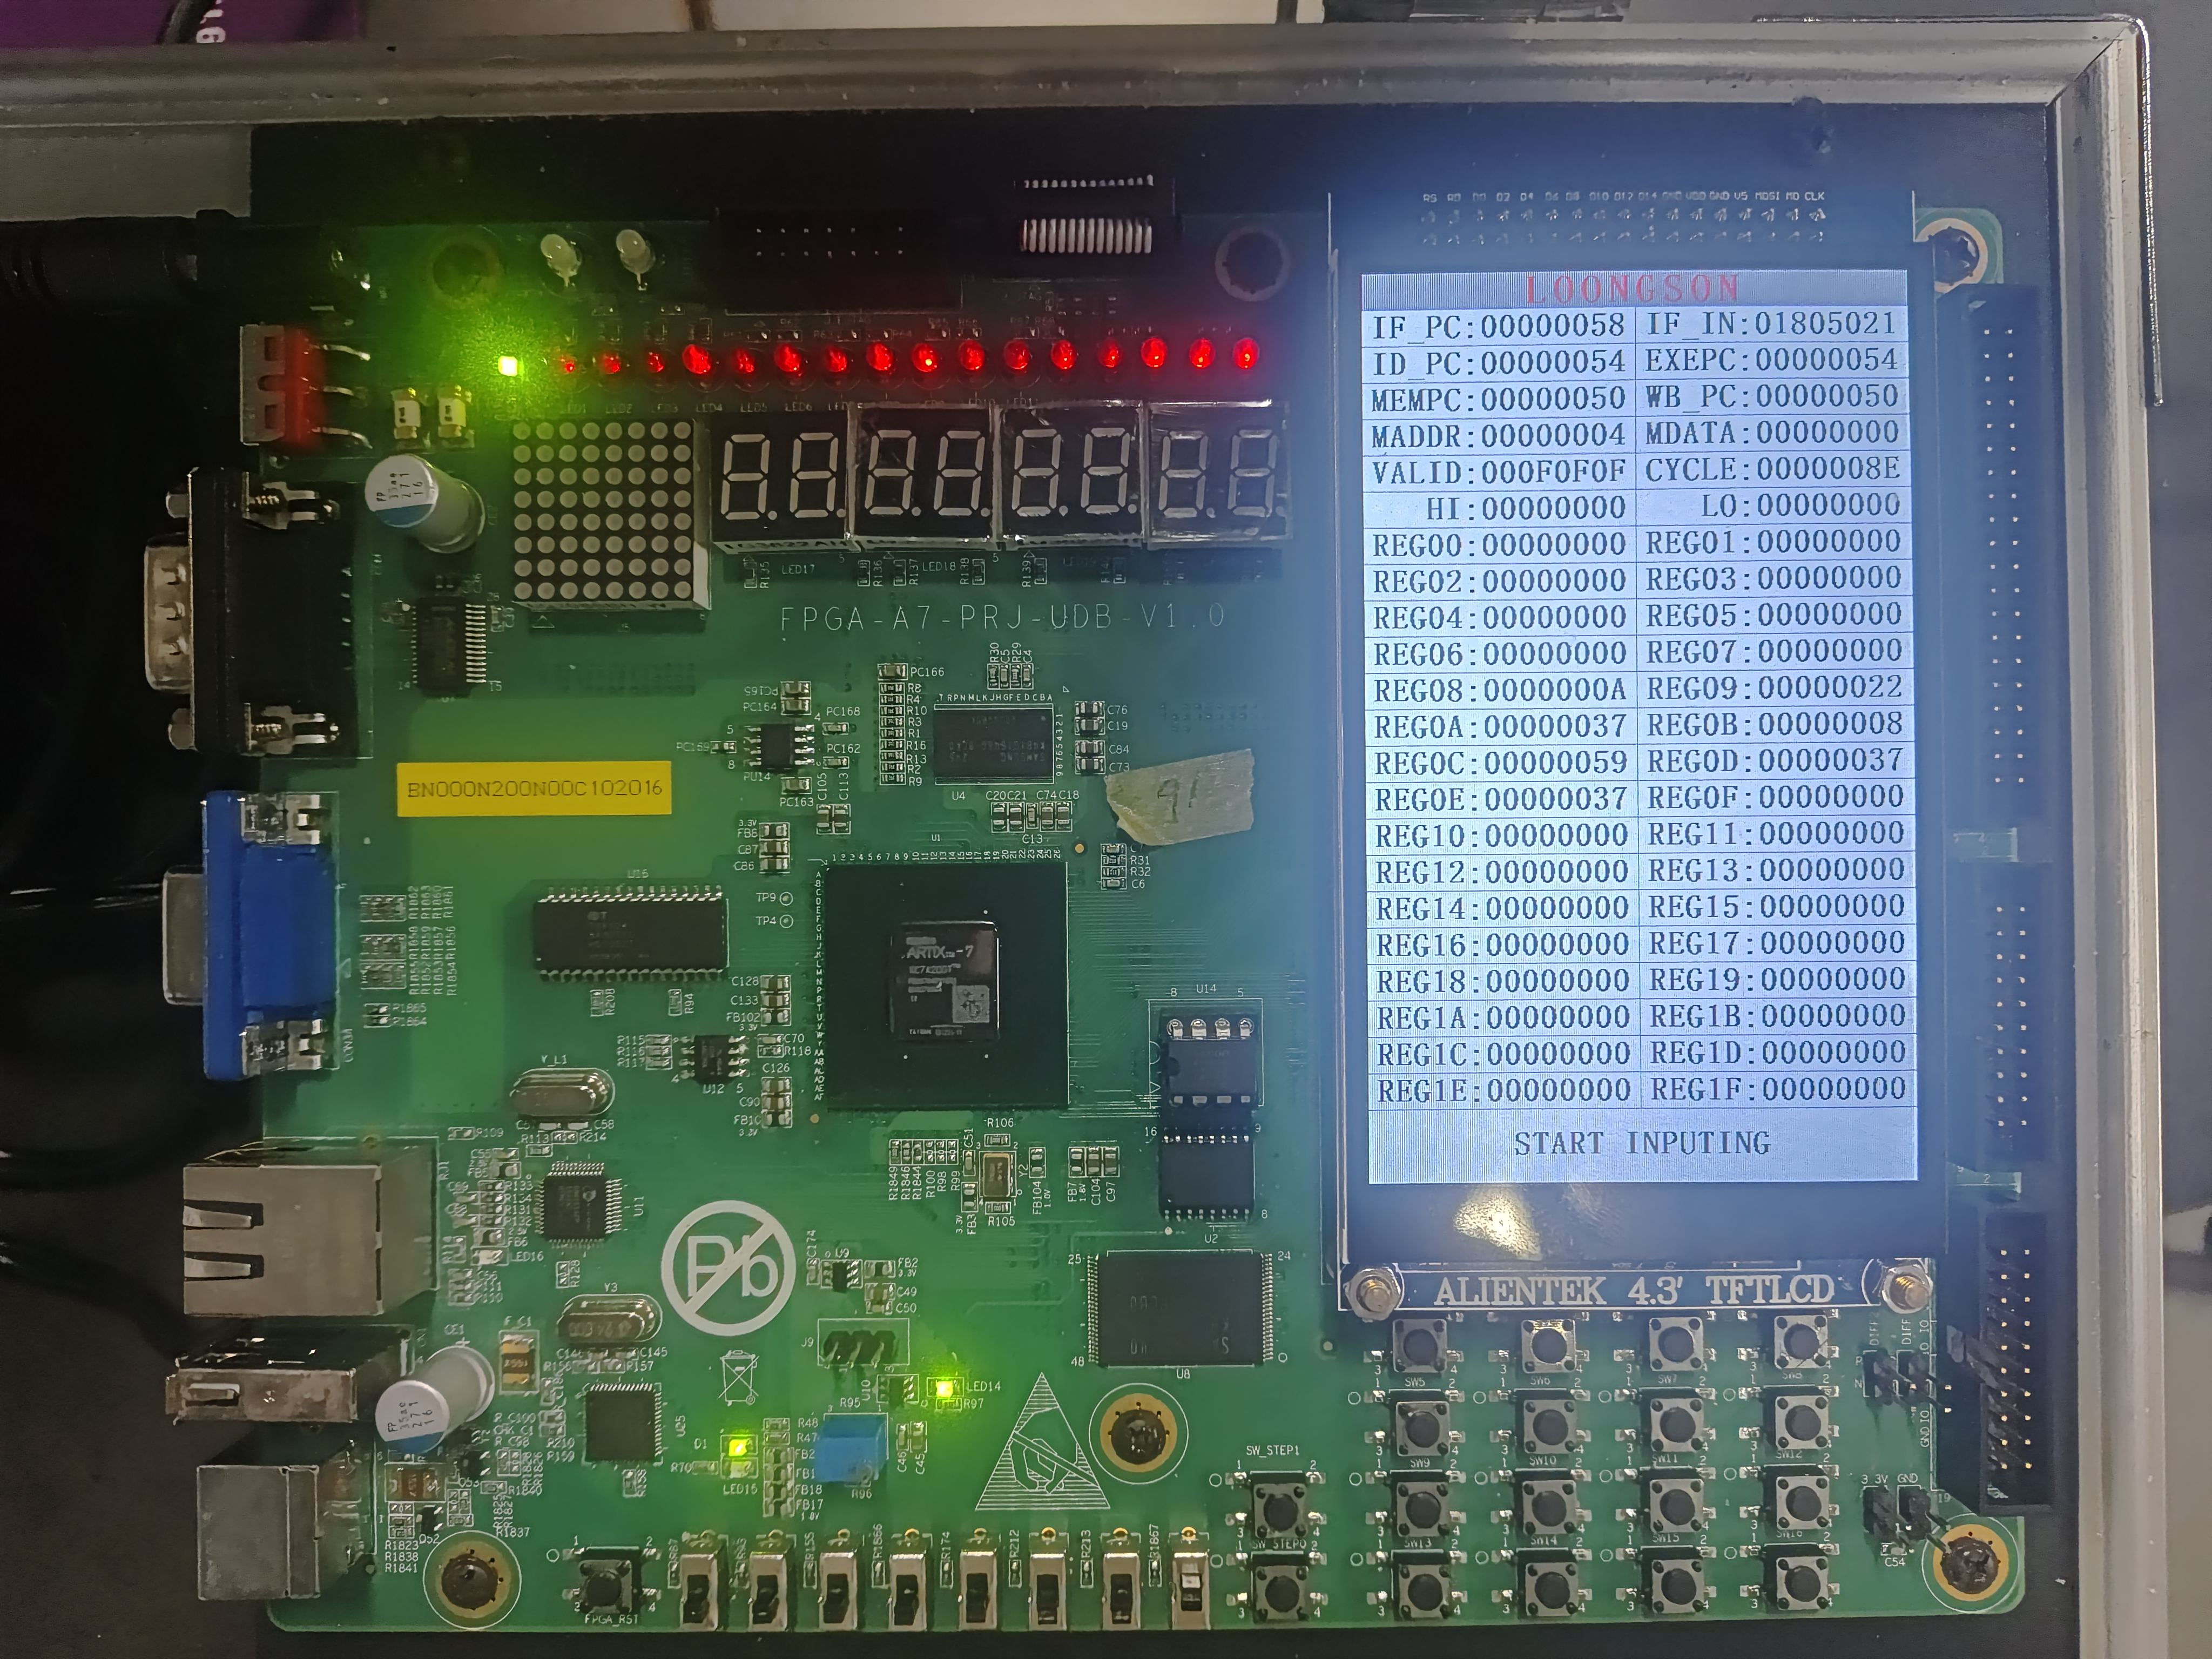
\includegraphics[width=\textwidth]{pipeline_fib.jpg}
  \caption{五级流水线CPU计算Fib(10)}
\end{figure}

可以从LCD屏上读取，计算得到斐波那契数列第10项，也即55（十六进制下为37）并将其写回内存Mem[1]，
五级流水线CPU消耗的周期数为8E（142）。指令ROM是同步读, PC更新后，下一拍才能拿到指令
。所以IF级本身就要2个周期，这意味着当前流水线的取指吞吐率上限不是 1 IPC，而更接近每2个周期取到1条新指令
，于是理论下界大概就是：68 × 2 + 4 = 140。

实验结果证明了以流水线的方式提高指令级并行度可以缩短程序的运行时间，提升硬件的利用效率。

\section{实验收获}
\begin{itemize}
  \item 实操了同步ROM和RAM IP核的创建
  \item 尝试了将汇编程序转换成coe文件预写入指令ROM
  \item 深入学习了五级流水线CPU的硬件描述实现
\end{itemize}

\end{document}
